\documentclass[a4paper,14pt]{extreport}

\usepackage[T2A]{fontenc}
\usepackage[utf8]{inputenc}
\usepackage[russian]{babel}
\usepackage{graphicx}
\usepackage{fontspec}
\usepackage{caption}
\usepackage{subcaption}
\setmainfont{Times New Roman} % мега кринж...

\usepackage[left=1cm,right=1cm,bottom=1cm,top=2cm]{geometry}
\usepackage{setspace}
\title{Меценаты Республики Карелия}
\author{Егор Федоров, P3115}
\date{Октябрь 2022 г.}

\usepackage{fancyhdr}
\fancyhead[L]{Федоров Егор, P3115}
\fancyhead[R]{Меценаты Республики Карелия}
\fancyfoot{}

\begin{document}
\pagestyle{fancy}
% \maketitle

\onehalfspacing{
\textbf{Камнеобрабатывающее предприятие <<Петрогранит>>} 24 июля 2020 г. профинансировала открытие
парка <<Аквамарин>> на набережной Варкауса.
В сквере высажено 10 голубых елей, 100 обыкновенных, 5 горных сосен, 5 яблонь, 58 спирей, 4 сирени.
В <<Аквамарине>> также установлены питьевой фонтан, небольшой водопад, скамейки, урны, спортивные тренажеры.
Для поддержания порядка в сквере установили камеры видеонаблюдения.

\begin{figure}[ht]
    \centering
    \begin{subfigure}[b]{0.3\textwidth}
        \centering
        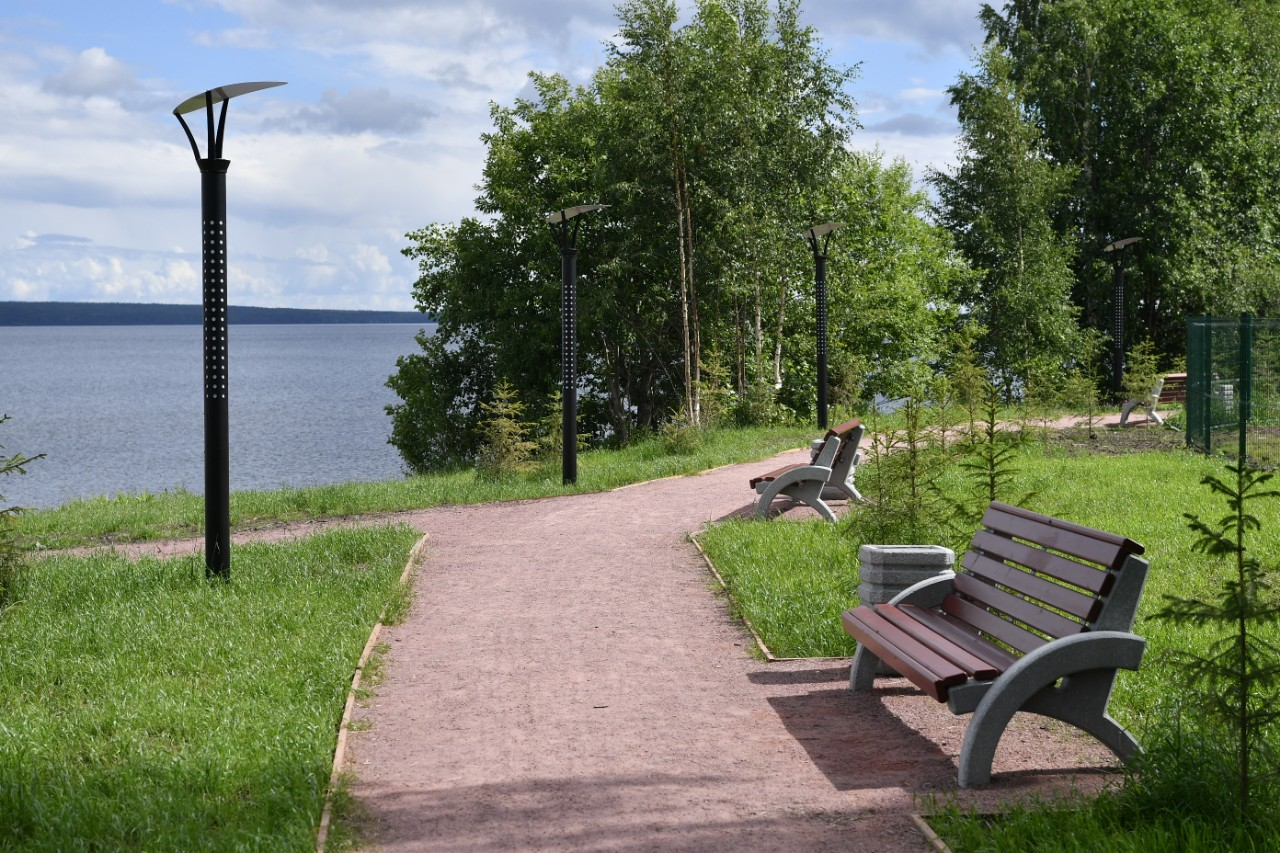
\includegraphics[width=\textwidth]{img/aqua1.jpg}
    \end{subfigure}
    \begin{subfigure}[b]{0.3\textwidth}
        \centering
        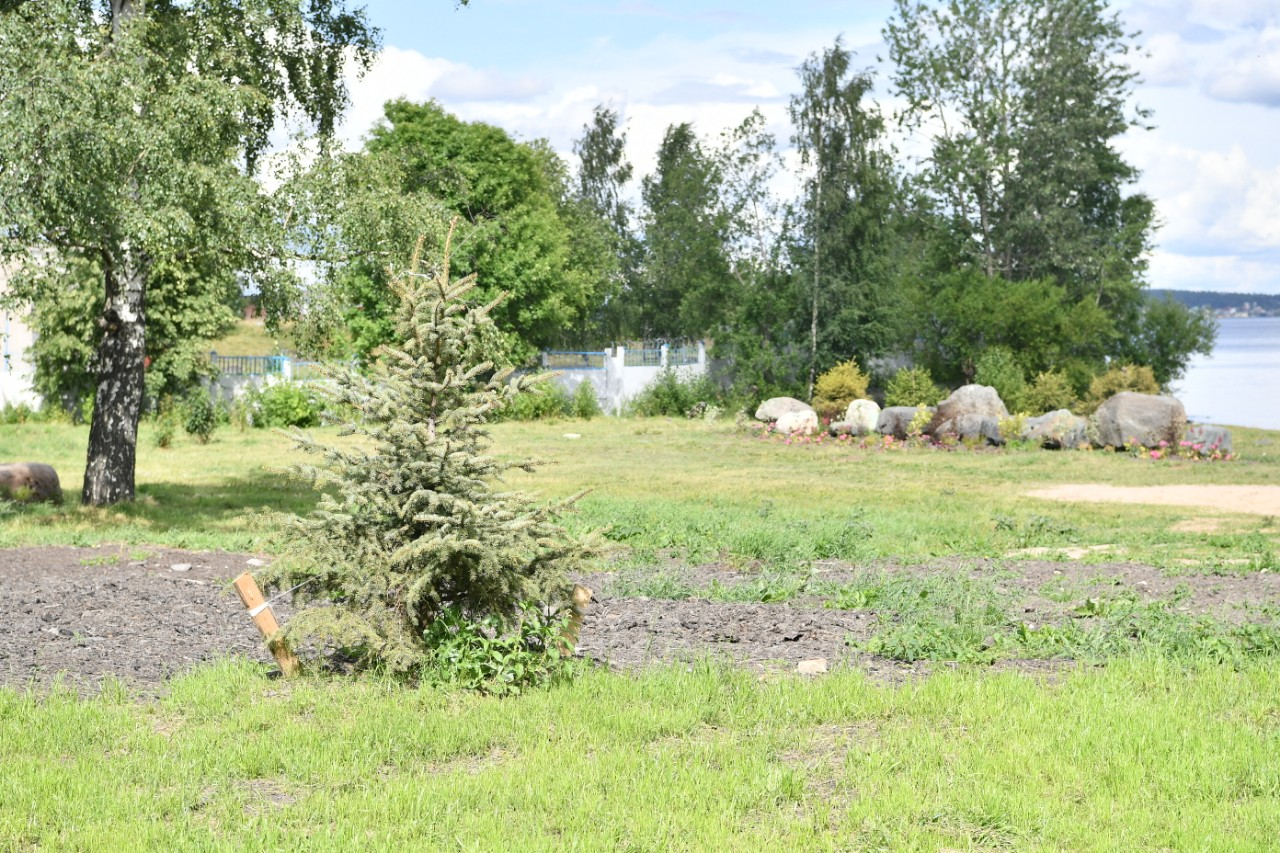
\includegraphics[width=\textwidth]{img/aqua2.jpg}
    \end{subfigure}
    \begin{subfigure}[b]{0.3\textwidth}
        \centering
        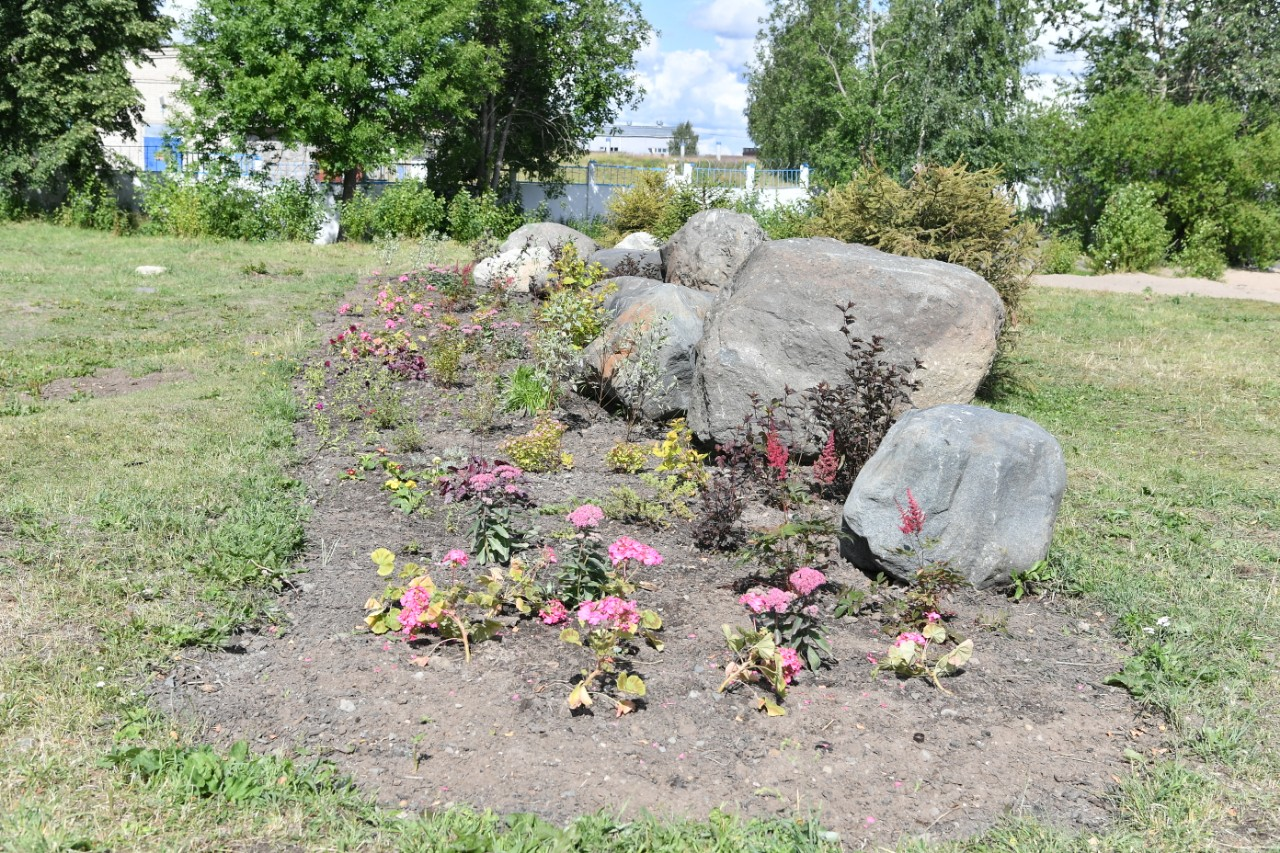
\includegraphics[width=\textwidth]{img/aqua3.jpg}
    \end{subfigure}
    \caption*{Парк <<Аквамарин>>}
\end{figure}


Компания <<Петрогранит>> также занимается обустройством лыжной трассы <<Фонтаны>>.
В планах компании превратить её в круглогодичный спортобъект.
Ранее за счет компании были сделаны два мостовых перехода.
Зимой 2020 года под автостоянку расчистили поляну на въезде на трассу.

\begin{figure}[ht]
    \centering
    \begin{subfigure}[b]{0.3\textwidth}
        \centering
        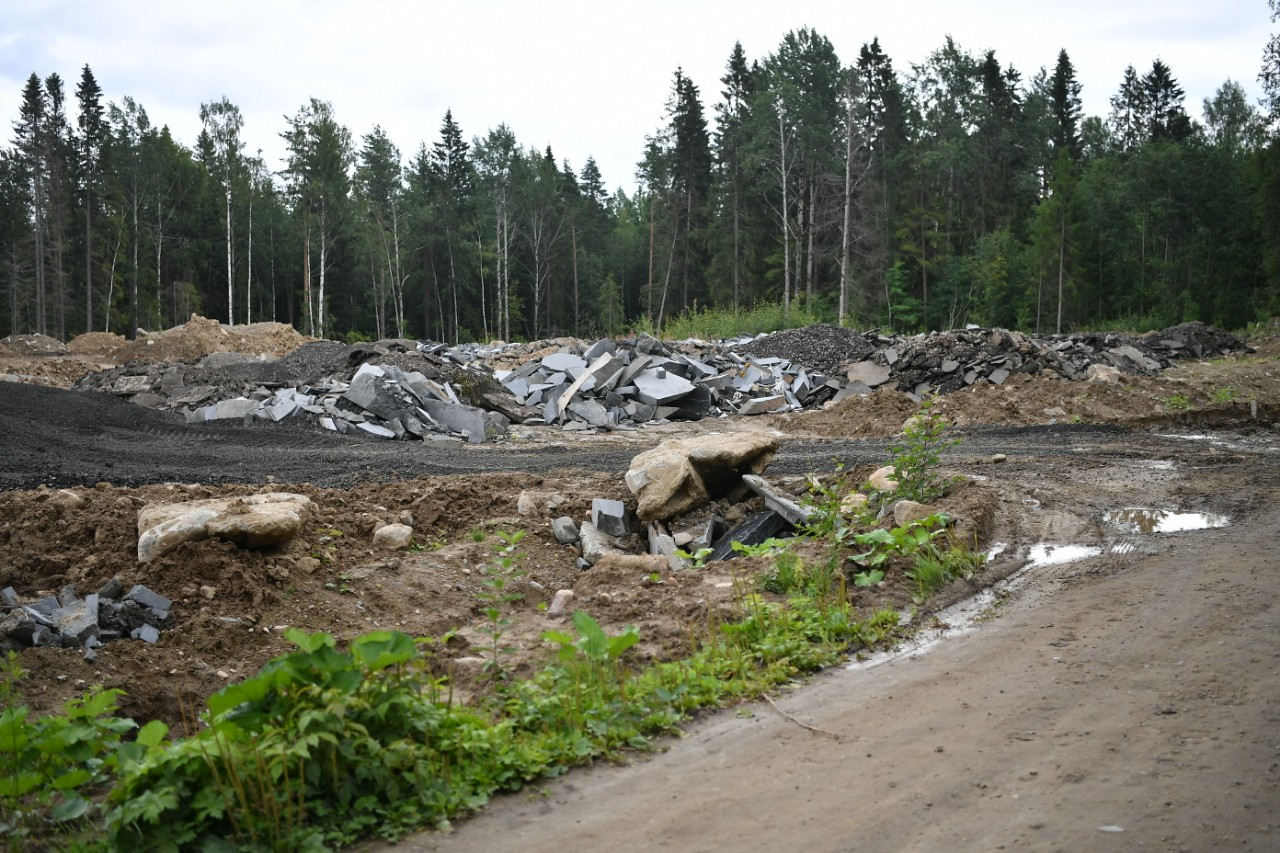
\includegraphics[width=\textwidth]{img/fountains1.jpg}
    \end{subfigure}
    \begin{subfigure}[b]{0.3\textwidth}
        \centering
        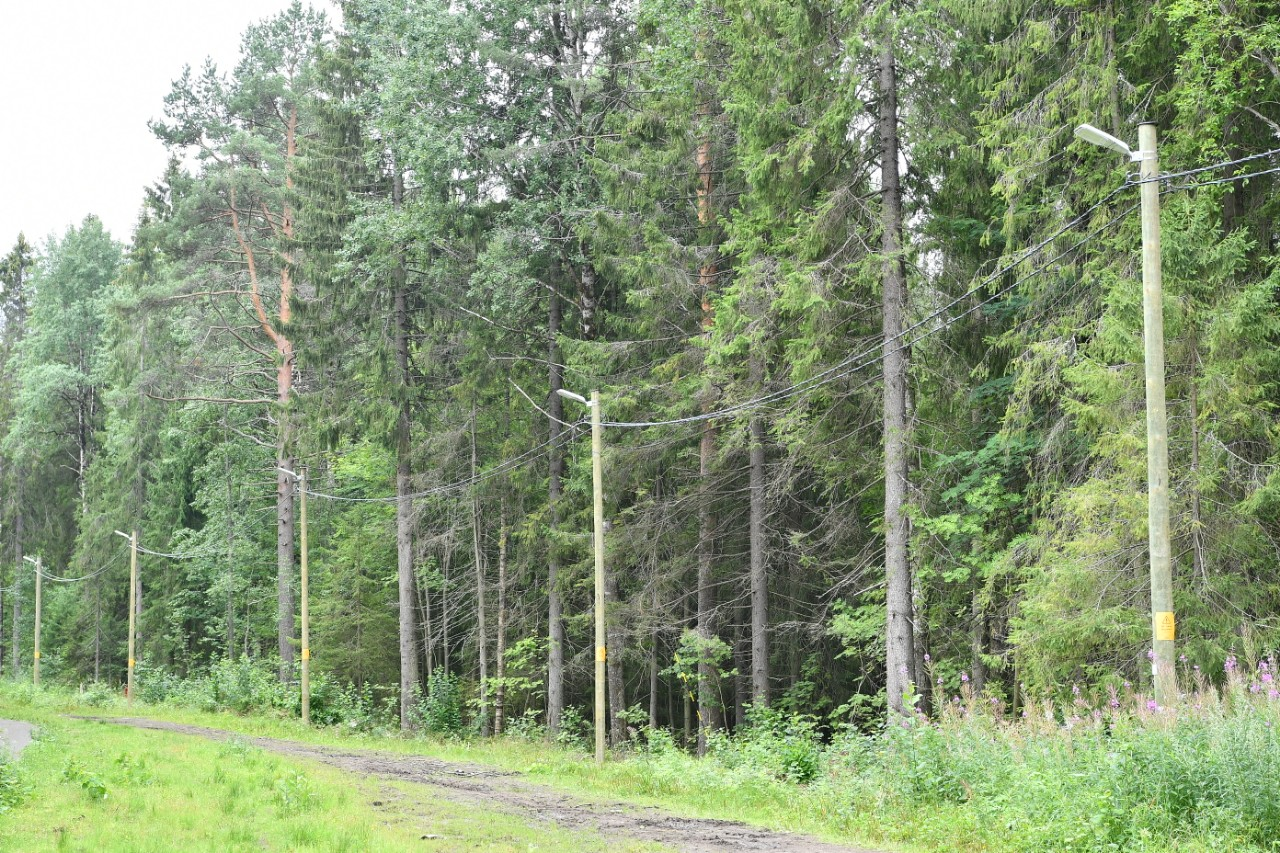
\includegraphics[width=\textwidth]{img/fountains2.jpg}
    \end{subfigure}
    \begin{subfigure}[b]{0.3\textwidth}
        \centering
        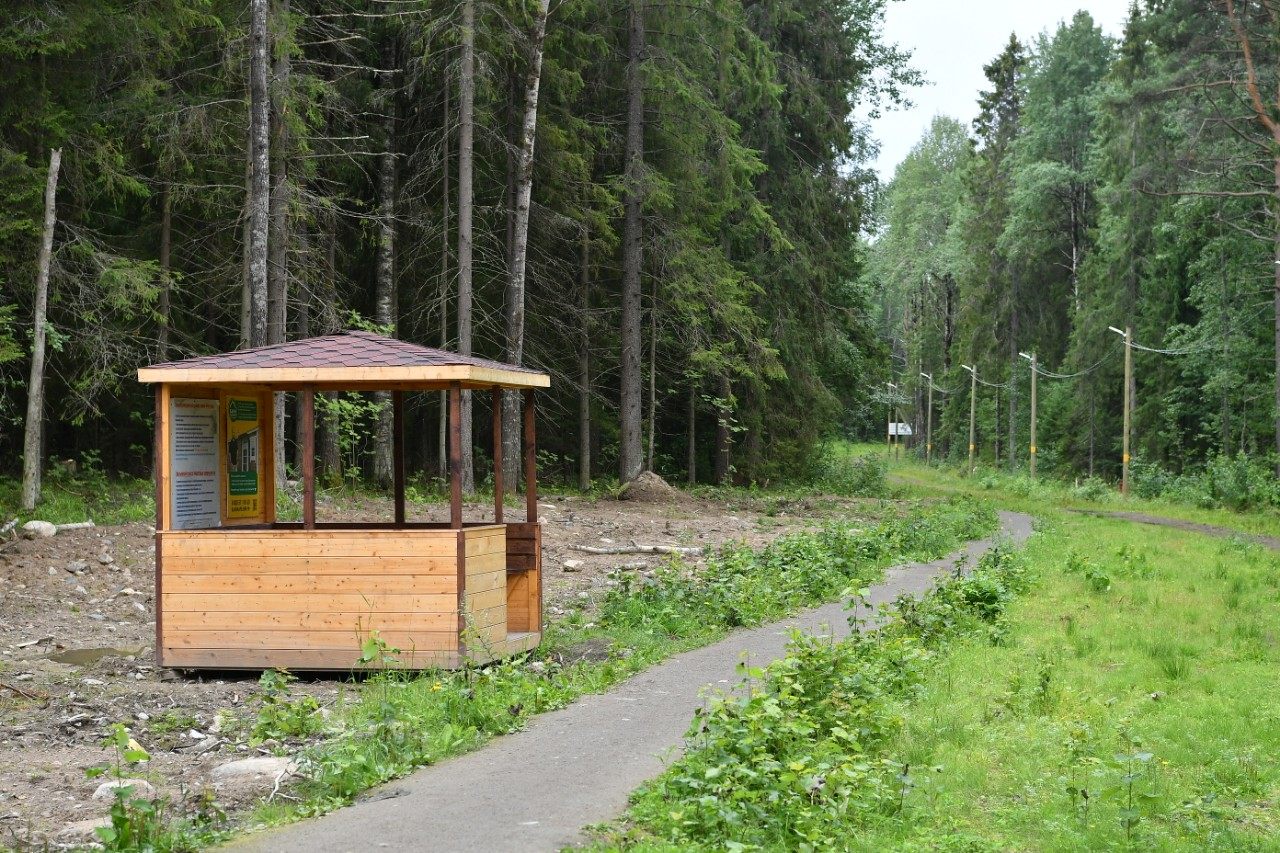
\includegraphics[width=\textwidth]{img/fountains3.jpg}
    \end{subfigure}
    \caption*{Трасса <<Фонтаны>>}
\end{figure}

\textbf{Иван Иванович Малокрошечный} (1808 --- 1870) --- российский купец первой гильдии, льнопромышленник, общественный деятель, благотворитель,
городской глава Пудожа (1859 --- 1862).

В 1859 г. построил на собственные средства православную церковь в с. Лекса Повенецкого уезда, с 1851 г. состоял попечителем Пудожской уездной больницы.

В 1863 г. купец пожертвовал 10 тыс. руб. на возрождение старинного Свято-Успенского Муромского монастыря в Пудожском уезде. 
На свои средства построил богадельню в Пудоже и давал деньги на ее содержание.

\end{document}